\documentclass{article}
\usepackage[utf8]{inputenc}
\usepackage[left=3cm, right=3cm, top=2cm]{geometry}
\title{Stability conditions and von Neumann Analysis}
\author{Silvin Willemsen}
\date{March 2019}
\usepackage{natbib}
\usepackage{graphicx}
\usepackage{appendix}
\usepackage{amsmath}
\usepackage{amsfonts}
\usepackage{amssymb}
\usepackage{xcolor} 
\def\SWcomment[#1]{\textcolor{blue}{#1}}

\begin{document}

\maketitle

\section{Introduction}
In this document I will show the calculations for different von Neumann analyses and stability conditions. The references to sections and equations with chapter numbers in them  (fx. (6.38) instead of fx. (9)) can be found in  Stefan Bilbao's Numerical Sound Synthesis book \cite{Bilbao2009}. Some background on this technique can be found in \cite{Strikwerda1989}.

% \begin{figure}[h!]
% \centering
% 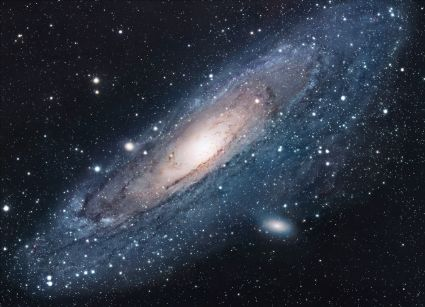
\includegraphics[scale=1.7]{universe}
% \caption{The Universe}
% \label{fig:universe}
% \end{figure}
\section{Identities}

\begin{equation}\label{eq:sinIdentity}
    \sin(x) = \frac{e^{jx} - e^{-jx}}{2j}\quad \Longrightarrow \quad \sin^2(x) = \frac{e^{j2x} - 2e^{jx-jx}+ e^{-j2x}}{-4} = \frac{e^{j2x} + e^{-j2x}}{-4} + \frac{1}{2}.
\end{equation}
From this we can derive the useful identity for $\sin^4(x)$:

\begin{align}
    \sin^4(x) = (\sin^2(x))^2 &= \Bigg(\frac{e^{j2x} + e^{-j2x}}{-4} + \frac{1}{2}\Bigg)^2\nonumber\\
    &=\Bigg(\frac{e^{j2x} + e^{-j2x}}{-4}\Bigg)^2 + \frac{e^{j2x} + e^{-j2x}}{-4} + \frac{1}{4}\nonumber\\
    &=\frac{e^{j4x} + e^{-j4x}}{16} + \frac{1}{8} + \underbrace{\frac{e^{j2x} + e^{-j2x}}{-4}}_\text{$\sin^2(x)- \frac{1}{2}$} + \frac{1}{4}\nonumber\\
    &= -\frac{1}{4}\Bigg(\frac{e^{j4x} + e^{-j4x}}{-4} + \frac{1}{2}\Bigg) + \frac{2}{8} + \sin^2(x) - \frac{1}{2} + \frac{1}{4}\nonumber\\
    &= -\frac{1}{4}\sin^2(2x) + \sin^2(x) \label{eq:sin4}
\end{align}
\subsection{Frequency domain analysis}
See section 5.2.6 of \cite{Bilbao2009}:
\begin{equation}
    u_l^n = z^n e^{jl\beta h}
\end{equation}
where $\beta$ is a real wavenumber. Important to remember is that without a shift in space (fx. $l+1$) or time (fx. $n-1$) $l = 0$ or $n=0$ respectively:
\begin{subequations} \label{eq:identitiesZ}
    \begin{align}
        u_l^n &= z^0 e^{j0\beta h} = 1\\
        u_{l+1}^n &= z^0 e^{j1\beta h} = e^{j\beta h}\\
        u_{l-1}^n &= z^0 e^{j(-1)\beta h} = e^{-j\beta h}\\
        u_{l+2}^n &= z^0 e^{j2\beta h} = e^{j\beta h}\\
        u_{l-2}^n &= z^0 e^{j(-2)\beta h}= e^{-j2\beta h}\\
        u_l^{n+1}&= z^1 e^{j0\beta h} = z\\
        u_l^{n-1}&= z^{-1} e^{j0\beta h} = z^{-1}
    \end{align}
\end{subequations}

\section{1D Wave Equation}
This section will derive the stability condition for the 1D wave equation. Starting from the FDS (Eq. 6.35)
\begin{equation}
    u_l^{n+1} = 2(1-\lambda^2)u_l^n + \lambda^2(u_{l+1}^n+u_{l-1}^n)-u_l^{n-1},
\end{equation}
where
\begin{equation}\label{eq:lambda}
    \lambda = \frac{ck}{h} \quad \text{and wave speed} \quad c = \sqrt{\frac{T}{\rho A}},
\end{equation}
with tension $T$, material density $\rho$ and cross-sectional area $A$.
We can now perform frequency domain analysis. Moving all terms to the left of the equals-sign and with their respective identities found in Eqs. \eqref{eq:identitiesZ} filled in, we get:
\begin{equation}\label{eq:zFDS}
    z - 2(1-\lambda^2)1 - \lambda^2(e^{j\beta h}+e^{-j\beta h}) + z^{-1} = 0.
\end{equation}
Using the identity found in Eq. \eqref{eq:sinIdentity} with $\beta h = 2x \Rightarrow x = \beta h / 2$ we can rewrite \eqref{eq:zFDS} to:
\begin{equation}
     z - 2 + 2\lambda^2 +4\lambda^2(\sin^2({\beta h / 2}) - 1/2) - z^{-1} = 0,
\end{equation}
and rewriting this yields the characterstic equation shown in Eq. (6.38):
\begin{equation}\label{eq:characteristic1D}
     z + 2(2\lambda^2\sin^2(\beta h/2) - 1) + z^{-1} = 0.
\end{equation}
The roots are then given by (using $X = \lambda^2\sin^2(\beta h/2)$):
\begin{equation}
\begin{aligned}\nonumber
    z_\pm &= \frac{-2(2X-1) \pm \sqrt{4(2X-1)^2 - 4 \cdot 1 \cdot 1}}{2}\\
    &= 1-2X \pm 1/2 \cdot \sqrt{4(2X-1)^2 - 4}\\
    &= 1-2X \pm 1/2 \cdot \sqrt{4(4X^2-4X + 1) - 4}\\
    &= 1-2X \pm 1/2 \cdot \sqrt{(4(4X^2 - 4X) + 4 - 4}\\
    &= 1-2X \pm 1/2 \cdot \sqrt{4(4X^2 - 4X)}\\
    &= 1-2X \pm 1/2 \cdot 2 \cdot \sqrt{4X^2 - 4X}\\
    &= 1-2X \pm \sqrt{(1 - 2X)^2 - 1}\\
\end{aligned}
\end{equation}
which results in the equation for the roots (right below (6.38) in section 6.2.2):
\begin{equation}
    z_\pm = 1-2\lambda^2\sin^2(\beta h/2) \pm \sqrt{(1 - 2\lambda^2\sin^2(\beta h/2))^2 - 1}.
\end{equation}
The scheme is then stable when these roots are bounded by unity for all $\beta$ \cite{BilbaoTutorial2018}
\begin{equation}\label{eq:boundByUnity}
    |z| \leq 1.
\end{equation} 
It can be shown that for a polynomial of the form 
\begin{equation}\label{eq:polynomialForm}
    z^2 + a^{(1)}z + a^{(2)}
\end{equation} it follows condition \eqref{eq:boundByUnity} when it abides the following (Eq. 2.14)
\begin{equation}\label{eq:condition214}
    |a^{(1)}| - 1 \leq a^{(2)} \leq 1,
\end{equation}
and when applied to the characteristic equation \eqref{eq:characteristic1D} (after multiplication with $z$), it can be seen that
\begin{equation}\nonumber
    \begin{aligned}
        |2(2\lambda^2\sin^2(\beta h/2) - 1)|-1 &\leq 1\\
        |2(2\lambda^2\sin^2(\beta h/2) - 1)| &\leq 2\\
        |2\lambda^2\sin^2(\beta h/2) - 1| &\leq 1,
    \end{aligned}    
\end{equation}
which is the equation right above Eq. (6.39). This can then be rewritten as
\begin{equation}\nonumber
    \begin{aligned}
        -1 \leq 2\lambda^2\sin^2(\beta h/2) - 1 &\leq 1\\
        0 \leq 2\lambda^2\sin^2(\beta h/2)&\leq 2\\
        0\leq \lambda^2\sin^2(\beta h/2) &\leq 1
    \end{aligned}
\end{equation}
and observing that all terms are squared, the result will always be non-negative, yielding Eq. (6.39):
\begin{equation}
     \lambda^2\sin^2(\beta h/2) \leq 1.
\end{equation}
Furthermore, knowing that the $\sin^2(\beta h / 2)$-term is bounded by $1$ for all $\beta$ the following condition is sufficient for stability (Eq. 6.40):
\begin{equation}
    \lambda \leq 1.
\end{equation}
Recalling \eqref{eq:lambda}, we see that the grid spacing is bounded by the following condition:
\begin{equation}
    h \geq h_\text{min} = ck.
\end{equation}
The closer $h$ is to $h_\text{min}$, the higher the quality of the implementation. 
\section{Ideal Bar}
Starting with the update equation for the ideal bar (eq. 7.12):
\begin{equation}
    u_l^{n+1}=(2-6\mu^2)u_l^n+4\mu^2(u_{l+1}^n+u_{l-1}^n)-\mu^2(u_{l+2}^n+u_{l-2}^n)-u_l^{n-1},
\end{equation}
where 
\begin{equation}\label{eq:mu}
    \mu = \frac{\kappa k}{h^2} \quad \text{and} \quad \kappa = \sqrt{\frac{EI}{\rho A}},
\end{equation}
we can perform frequency domain analysis by filling in the identities from Eqs. \eqref{eq:identitiesZ} yielding
\begin{equation}\label{eq:zFDSBar}
    z-2+6\mu^2-4\mu^2(e^{j\beta h}+e^{-j\beta h}) + \mu^2 (e^{j2\beta h}+e^{-j2\beta h}) + z^{-1} = 0.
\end{equation}
Again, using the identity found in Eq. \eqref{eq:sinIdentity} with $\beta h = 2x \Rightarrow x = \beta h / 2$ we can rewrite \eqref{eq:zFDSBar} to

\begin{equation}\nonumber
    \begin{aligned}
        &z-2+6\mu^2+16\mu^2(\sin^2(\beta h / 2)) - 8\mu^2  -4 \mu^2 (\sin^2(\beta h)) + 2\mu^2 + z^{-1} = 0\\
        &z-2+16\mu^2(\sin^2(\beta h / 2)) -4 \mu^2 (\sin^2(\beta h)) + z^{-1} = 0.
    \end{aligned}  
\end{equation}
We can rewrite the above to
\begin{equation}\nonumber
    z-2+16\mu^2\bigg(-\frac{1}{4}\sin^2(\beta h)+\sin^2(\beta h / 2)\bigg) + z^{-1} = 0,
\end{equation}
and using Eq. \eqref{eq:sin4} we can simplify this to the characteristic equation (Eq. (7.13))

\begin{equation}
    z+(16\mu^2\sin^4(\beta h/2) - 2) + z^{-1} = 0.
\end{equation}
The parentheses are used here to denote that $16\mu^2\sin^4(\beta h/2) - 2$ is a single term ($a^{(1)}$) in condition \eqref{eq:condition214}. Using this condition we get
\begin{equation}\nonumber
    \begin{aligned}
        |16\mu^2\sin^4(\beta h/2) - 2|-1&\leq 1\\
        |8\mu^2\sin^4(\beta h/2) - 1|&\leq 1\\
        -1\leq8\mu^2\sin^4(\beta h/2) - 1&\leq 1\\
        0\leq8\mu^2\sin^4(\beta h/2)&\leq 2\\
        0\leq\mu^2\sin^4(\beta h/2)&\leq \frac{1}{4},
    \end{aligned}
\end{equation}
and as the $\sin^4(\beta h/2)$-term is again bounded by 1 and observing that all terms are squared, so non-negative, we get Eq. (7.14)
\begin{equation}
    \mu^2 \leq \frac{1}{4}\quad \Longleftrightarrow\quad \mu \leq \frac{1}{2}.
\end{equation}
Recalling \eqref{eq:mu} we get the stability condition in terms of grid spacing $h$ 
    \begin{equation}
    \frac{\kappa k}{h^2}\leq \frac{1}{2}\quad \Longleftrightarrow\quad h \geq h_\text{min} = \sqrt{2\kappa k}.
\end{equation}

\section{Stiff String}
The characteristic equation for the stiff string, after obtaining the following update equation
\begin{equation}
    u_l^{n+1}=(2-2\lambda^2-6\mu^2)u_l^n+(\lambda^2+4\mu^2)(u_{l+1}^n+u_{l-1}^n)-\mu^2(u_{l+2}^n+u_{l-2}^n)-u_l^{n-1}
\end{equation}
can, after frequency domain analysis, be shown to be
\begin{equation}
    z + (4\lambda^2\sin^2(\beta h/2)+16\mu^2\sin^4(\beta h/2)-2) +z^{-1} = 0.
\end{equation}
Using \eqref{eq:condition214} and solving the inequality in terms of $\lambda$ and $\mu$ we get
\begin{equation}\label{eq:stiffStringInequality}
    \begin{aligned}
    |4\lambda^2\sin^2(\beta h/2)+16\mu^2\sin^4(\beta h/2)-2|-1&\leq 1\\
    0\leq\lambda^2\sin^2(\beta h/2)+4\mu^2\sin^4(\beta h/2)&\leq 1,
    \end{aligned}
\end{equation}
which, after observing the $\sin$-terms to be bounded by 1 and non-negativity of the solution through the squared terms, we obtain Eq. (7.24)
\begin{equation}
    \lambda^2+4\mu^2\leq 1.
\end{equation}
Recalling \eqref{eq:lambda} and \eqref{eq:mu}, we can write
\begin{equation}
    \begin{aligned}
        \frac{c^2k^2}{h^2} + 4 \frac{\kappa^2h^2}{h^4}\leq 1\\
        h^4 - c^2k^2h^2-4\kappa^2k^2 \geq 0,
    \end{aligned}
\end{equation}
and the minimum stable value for $h$ can be found

\begin{equation}
    h \geq h_\text{min} = \sqrt{\frac{c^2k^2+\sqrt{c^4k^4+16\kappa^2k^2}}{2}}.
\end{equation}
\subsection{Adding Damping}\label{sec:dampedString}
Adding damping to the stiff string will result in the following update equation:
\begin{equation}\label{eq:dampedStiffString}
    \begin{aligned}
    (1+\sigma_0k)u_l^{n+1} &= (2-2\lambda^2-6\mu^2-\frac{4\sigma_1k}{h^2})u_l^n +(\lambda^2 + 4\mu^2 + \frac{2\sigma_1k}{h^2})(u_{l+1}^n+u_{l-1}^n)\\
    &-\mu^2(u_{l+2}^n+u_{l-2}^n)+(-1 + \sigma_0k+\frac{4\sigma_1k}{h^2})u_l^{n-1} -\frac{2\sigma_1k}{h^2}(u_{l+1}^{n-1}+u_{l-1}^{n-1}),
    \end{aligned}
\end{equation}
where $\sigma_0 \geq 0$ and $\sigma_1\geq0$ are the frequency independent and frequency dependent damping respectively. The characteristic equation of \eqref{eq:dampedStiffString} can be shown to be
\begin{equation}\label{eq:charDampedString}
    (1+\sigma_0k)z + \bigg(16\mu^2\sin^4(\beta h/2)+(4\lambda^2+\frac{8\sigma_1k}{h^2})\sin^2(\beta h/2) - 2\bigg)+\bigg(1-\sigma_0k-\frac{8\sigma_1k}{h^2}\sin^2(\beta h/2)\bigg)z^{-1}=0.
\end{equation}
Dividing by $(1+\sigma_0k)$ to get a polynomial of the form presented in \eqref{eq:polynomialForm} and employing \eqref{eq:condition214} yields

\begin{equation}\nonumber
    \begin{aligned}
        &\Bigg|\frac{16\mu^2\sin^4(\beta h/2)+(4\lambda^2+\frac{8\sigma_1k}{h^2})\sin^2(\beta h/2) - 2}{1+\sigma_0k}\Bigg|-1 \leq \frac{1-\sigma_0k-\frac{8\sigma_1k}{h^2}\sin^2(\beta h/2)}{1+\sigma_0k}\leq 1\\
        &\Bigg|16\mu^2\sin^4(\beta h/2)+(4\lambda^2+\frac{8\sigma_1k}{h^2})\sin^2(\beta h/2) - 2\Bigg|-(1+\sigma_0k) \leq 1-\sigma_0k-\frac{8\sigma_1k}{h^2}\sin^2(\beta h/2)\leq 1+\sigma_0k\\
        &\Big|16\mu^2\sin^4(\beta h/2)+(4\lambda^2+\frac{8\sigma_1k}{h^2})\sin^2(\beta h/2) - 2\Big|\leq2-\frac{8\sigma_1k}{h^2}\sin^2(\beta h/2)\leq2+2\sigma_0k\\
        &\Big|16\mu^2\sin^4(\beta h/2)+(4\lambda^2+\frac{8\sigma_1k}{h^2})\sin^2(\beta h/2) - 2\Big|-2\leq-\frac{8\sigma_1k}{h^2}\sin^2(\beta h/2)\leq2\sigma_0k.
    \end{aligned}
\end{equation}
% \SWcomment[Something wrong here with $\sigma_0$] Assuming the lowest possible value for $\sigma_0$ (which is 0) and subtracting 2 from all, we get the following inequality
The last inequality is always true due to the fact that $\sigma_0,\sigma_1 \geq 0$.  
\begin{equation}
        \Big|16\mu^2\sin^4(\beta h/2)+(4\lambda^2+\frac{8\sigma_1k}{h^2})\sin^2(\beta h/2) - 2\Big|-2\leq-\frac{8\sigma_1k}{h^2}\sin^2(\beta h/2)\leq0.
\end{equation}
It can be concluded that the last inequality will be satisfied for any value of $\beta$, i.e., $-\frac{8\sigma_1k}{h^2}\sin^2(\beta h/2)$ will always be less or equal to zero. Removing this inequality and continuing the derivation gives
\begin{equation}
    0 \leq 16\mu^2\sin^4(\beta h/2) + 4\lambda^2\sin^2(\beta h/2) \leq 4-\frac{16\sigma_1k}{h^2}\sin^2(\beta h/2).
\end{equation}
Again, we know that the first inequality will always be satisfied (squared terms), so disregarding this we can continue:
\begin{equation}
    \begin{aligned}
        4\mu^2\sin^4(\beta h/2) + \lambda^2\sin^2(\beta h/2)+\frac{4\sigma_1k}{h^2}\sin^2(\beta h/2) \leq 1.
    \end{aligned}
\end{equation}
Considering (again) the fact that the $\sin$-terms are bounded by 1 we get the condition
\begin{equation}
    4\mu^2 + \lambda^2 + \frac{4\sigma_1k}{h^2} \leq 1,
\end{equation}
which, again recalling \eqref{eq:lambda} and \eqref{eq:mu}, can be solved for the minimum stable value of $h$:
\begin{equation}
    \begin{aligned}
        &\frac{4\kappa^2k^2}{h^4}+\frac{c^2k^2+4\sigma_1k}{h^2} - 1 \leq 0,\\
        &h^4 - (c^2k^2+4\sigma_1k)h^2 - 4\kappa^2k^2 \geq 0,\\
        &h\geq h_\text{min} = \sqrt{\frac{c^2k^2+4\sigma_1k+\sqrt{(c^2k^2+4\sigma_1k)^2+16\kappa^2k^2}}{2}}.
    \end{aligned}
\end{equation}
\subsubsection{Alternatively..}
By only looking at the discrete and not-expanded PDE of the damped stiff string
\begin{equation}\label{eq:dampedStiffStringFDS}
    \delta_{tt}u=c^2\delta_{xx}u-\kappa^2\delta_{xxxx}u-2\sigma_0\delta_{t\cdot}u+2\sigma_1\delta_{t-}\delta_{xx}u,
\end{equation}
we can use the following identities (Eqs. 5.15a and 5.15b):
\begin{subequations}\label{eq:fourierIdentities}
\begin{align}
% \delta_{tt}u \overset{\mathcal{F}}{\Longrightarrow}-\frac{4}{k^2}sin^2n
    \delta_{xx}u \overset{\mathcal{F}}{\Longrightarrow} -\frac{4}{h^2}\sin^2(\beta h/2)\tilde{u}\\
    \delta_{xxxx}u \overset{\mathcal{F}}{\Longrightarrow} \frac{16}{h^4}\sin^4(\beta h/2)\tilde{u}
\end{align}
\end{subequations}
which, after frequency analysis yields
\begin{equation}
\begin{aligned}
    z - 2 + z^{-1} &= -4\lambda^2\sin^2(\beta h/2) - 16\mu^2\sin^4(\beta h/2) - \sigma_0kz + \sigma_0k z^{-1} \\
    &- \frac{8 \sigma_1 k}{h^2}\sin^2(\beta h/2) + \frac{8 \sigma_1 k}{h^2} \sin^2(\beta h/2)z^{-1}
    \end{aligned}
\end{equation}
and can be rewritten to characteristic equation \eqref{eq:charDampedString}.

\subsection{Centered Frequency Dependent Damping}
We can modify Eq. \eqref{eq:dampedStiffStringFDS} to have a centered-time rather than a backwards-time operator 
\begin{equation}
    \delta_{tt}u=c^2\delta_{xx}u-\kappa^2\delta_{xxxx}u-2\sigma_0\delta_{t\cdot}u+2\sigma_1\delta_{t\cdot}\delta_{xx}u.
\end{equation}
Although, this makes the scheme implicit, it has great properties with regards to stability as will be shown below. 

Using the identities in \eqref{eq:fourierIdentities} we get
\begin{equation}
\begin{aligned}
    z - 2 + z^{-1} &= -4\lambda^2\sin^2(\beta h/2) - 16\mu^2\sin^4(\beta h/2) - \sigma_0kz + \sigma_0k z^{-1} \\
    &- \frac{4 \sigma_1 k}{h^2}\sin^2(\beta h/2)z + \frac{4 \sigma_1 k}{h^2} \sin^2(\beta h/2)z^{-1}
    \end{aligned}
\end{equation}
which after refactoring yields the characteristic equation
\begin{equation}
    \begin{aligned}
        \left(1+\sigma_0k + \frac{4\sigma_1k}{h^2}\sin^2(\beta h/2)\right)z &+ \left(16\mu^2\sin^4(\beta h/2)+4\lambda^2\sin^2(\beta h/2) - 2\right)\\
        & + \left(1-\sigma_0k - \frac{4\sigma_1k}{h^2}\sin^2(\beta h/2)\right)z^{-1} = 0.
    \end{aligned}
\end{equation}
Then, again, written in the form \eqref{eq:polynomialForm} and employing \eqref{eq:condition214} yields
\begin{align*}
    &\left|\frac{16\mu^2\sin^4(\beta h/2)+4\lambda^2\sin^2(\beta h/2) - 2}{1+\sigma_0k + \frac{4\sigma_1k}{h^2}\sin^2(\beta h/2)} \right|-1 \leq \frac{1-\sigma_0k - \frac{4\sigma_1k}{h^2}\sin^2(\beta h/2)}{1+\sigma_0k + \frac{4\sigma_1k}{h^2}\sin^2(\beta h/2)}\leq 1\\
    &\left|16\mu^2\sin^4(\beta h/2)+4\lambda^2\sin^2(\beta h/2) - 2 \right|\leq1-\sigma_0k - \frac{4\sigma_1k}{h^2}\sin^2(\beta h/2)+ 1+\sigma_0k + \frac{4\sigma_1k}{h^2}\sin^2(\beta h/2)\\
    &\qquad\qquad\qquad\qquad\qquad\leq 2+2\sigma_0k + \frac{8\sigma_1k}{h^2}\sin^2(\beta h/2)\\
    &\left|16\mu^2\sin^4(\beta h/2)+4\lambda^2\sin^2(\beta h/2) - 2 \right|\leq 2 \leq 2+2\sigma_0k + \frac{8\sigma_1k}{h^2}\sin^2(\beta h/2)
\end{align*}
Notice that in the second step, all terms including damping cancel out, excluding $\sigma_1$ from the eventual stability condition. Also note that due to $\sigma_0, \sigma_1 \geq 0$, the last inequality is always satisfied leaving
\begin{equation}
    \left|16\mu^2\sin^4(\beta h/2)+4\lambda^2\sin^2(\beta h/2) - 2 \right|\leq 2
\end{equation}
which is identical to \eqref{eq:stiffStringInequality}.

To conclude, the stability condition for the damped stiff string where a centered-time difference operator is used for the frequency dependent damping is identical to that of the undamped stiff string.
\section{2D case: Damped Plate}
The FDS for a 2D (damped) plate is defined as the following:
\begin{equation}\label{eq:plateFDS}
    \delta_{tt}u = -\kappa^2\delta_{\Delta\boxplus}\delta_{\Delta\boxplus} u - 2\sigma_0\delta_{t\cdot}u + 2\sigma_1\delta_{t-}\delta_{\Delta\boxplus}u.
\end{equation}
We can use the following identities (the equations in (10.14)) for frequency analysis
\begin{align}
% \delta_{tt}u \overset{\mathcal{F}}{\Longrightarrow}-\frac{4}{k^2}sin^2n
    \delta_{\Delta\boxplus}u \overset{\mathcal{F}}{\Longrightarrow} -\frac{4}{h^2}(p_x + p_y)\tilde{u}\\
    \delta_{\Delta\boxplus}\delta_{\Delta\boxplus}u \overset{\mathcal{F}}{\Longrightarrow} \frac{16}{h^4}(p_x + p_y)^2\tilde{u}
\end{align}
where (Eq. (10.13))
\begin{equation}\label{eq:pxpy}
    p_x = \sin^2(\beta_xh/2) \quad \text{and} \quad p_y = \sin^2(\beta_yh/2)
\end{equation}
and write the following characteristic equation
\begin{equation}
    (1+\sigma_0k)z + \Big(16\mu^2(p_x+p_y)^2 + \frac{8\sigma_1k}{h^2}(p_x+p_y) - 2\Big) + (1 - \sigma_0k - \frac{8\sigma_1k}{h^2}(p_x+p_y))z^{-1} = 0.
\end{equation}
This can, similarly to the damped stiff string in Section \ref{sec:dampedString} of this document, be solved to
\begin{equation}
    4\mu^2(p_x+p_y)^2 + \frac{4\sigma_1k}{h^2}(p_x+p_y) \leq 1.
\end{equation}
Recalling \eqref{eq:pxpy}, and given the fact that these are bounded by 1, we can write the following
\begin{gather}
    4\mu^2(1+1)^2 + \frac{4\sigma_1k}{h^2}(1+1) \leq 1\nonumber\\
    16\mu^2 + \frac{8\sigma_1k}{h^2} \leq 1.
\end{gather}
Solving for $h$ then gives
\begin{align}
    &1 \geq \frac{16\kappa^2k^2}{h^4} + \frac{8\sigma_1k}{h^2}\nonumber\\
    &h^4 - 8\sigma_1kh^2 - 16\kappa^2k^2 \geq 0\nonumber\\
    &h \geq \sqrt{\frac{8\sigma_1k +\sqrt{(8\sigma_1k)^2 + 64\kappa^2k^2}}{2}}\nonumber\\
    &h\geq \sqrt{\frac{8\sigma_1k+8\sqrt{\sigma_1^2k^2+\kappa^2k^2}}{2}}\nonumber\\
    &h \geq 2\sqrt{k\left(\sigma_1 + \sqrt{\sigma_1^2 + \kappa^2}\right)}
\end{align}

\subsection{Adding tension (Stiff damped membrane)}
Adding a tension term to the plate above (Eq. \eqref{eq:plateFDS}) to make it a stiff damped membrane yields
\begin{equation}
    \delta_{tt}u = c^2\delta_{\Delta\boxplus}u -\kappa^2\delta_{\Delta\boxplus}\delta_{\Delta\boxplus} u - 2\sigma_0\delta_{t\cdot}u + 2\sigma_1\delta_{t-}\delta_{\Delta\boxplus}u.
\end{equation}
%
The characteristic equation will then be
\begin{equation}
    (1+\sigma_0k)z + \left(4\lambda^2(p_x+p_y)+16\mu^2(p_x+p_y)^2 + \frac{8\sigma_1k}{h^2}(p_x+p_y) - 2\right) + \left(1 - \sigma_0k - \frac{8\sigma_1k}{h^2}(p_x+p_y)\right)z^{-1} = 0,
\end{equation}
and can, similarly to the plate, be solved to
\begin{equation}
    \lambda^2(p_x+p_y)+4\mu^2(p_x+p_y)^2+\frac{4\sigma_1k}{h^2}(p_x+p_y)\leq 1.
\end{equation}
Again, recalling \eqref{eq:pxpy} and that these are bounded by 1, we can write
\begin{gather}
    \lambda^2(1+1)+4\mu^2(1+1)^2+\frac{4\sigma_1k}{h^2}(1+1)\leq 1\nonumber\\
    2\lambda^2+16\mu^2+\frac{8\sigma_1k}{h^2}\leq 1.
\end{gather}
Solving for $h$ then finally yields
\begin{align}
    h^4 - (2c^2k^2 + 8\sigma_1k)h^2 - 16\kappa^2k^2 \geq 0\nonumber\\
    h\geq \sqrt{\frac{2c^2k^2 + 8\sigma_1k+\sqrt{(2c^2k^2 + 8\sigma_1k)^2 + 64\kappa^2k^2}}{2}}\nonumber \\
    h\geq \sqrt{c^2k^2 + 4\sigma_1k+\frac{1}{2}\sqrt{4(c^2k^2 + 4\sigma_1k)^2 + 64\kappa^2k^2}}\nonumber\\
    h\geq \sqrt{c^2k^2 + 4\sigma_1k+\sqrt{(c^2k^2 + 4\sigma_1k)^2 + 16\kappa^2k^2}}
\end{align}
\bibliographystyle{plain}
\bibliography{references}
\appendix
\newpage
\section{Note on scaling}
Proof that calculating the stability condition in non-dimensionalised form is the same as the condition in dimensionalised form scaled by $\frac{1}{L}$, i.e., 
\begin{equation}
    h_\text{nd} = \frac{1}{L}h_\text{d}.
\end{equation}
Let's use the case of the undamped stiff string
\begin{align}
    h_\text{d} &= \sqrt{\frac{c^2k^2 + \sqrt{c^4k^4 + 16\kappa_\text{d}^2k^2}}{2}} \label{eq:hd}\\
    h_\text{nd} &= \sqrt{\frac{\gamma^2k^2 + \sqrt{\gamma^4k^4 + 16\kappa_\text{nd}^2k^2}}{2}}\label{eq:hnd}
\end{align}
with
\begin{equation}
    \gamma = \frac{c}{L}\quad \text{and}\quad \kappa_\text{nd} = \frac{\kappa_\text{d}}{L^2}.
\end{equation}

Substituting these definitions into \eqref{eq:hnd} yields
\begin{align}
    h_\text{nd} &= \sqrt{\frac{\frac{c^2}{L^2}k^2 + \sqrt{\frac{c^4}{L^4}k^4 + 16\frac{\kappa_\text{d}^2}{L^4}k^2}}{2}}\nonumber\\
    &= \sqrt{\frac{\frac{1}{L^2}c^2k^2 + \sqrt{\frac{1}{L^4}\left(c^4k^4 + 16\kappa_\text{d}^2k^2\right)}}{2}}\nonumber\\
    &= \sqrt{\frac{1}{L^2}\left(\frac{c^2k^2 + \sqrt{c^4k^4 + 16\kappa_\text{d}^2k^2}}{2}\right)}\nonumber\\
    &= \frac{1}{L}\sqrt{\left(\frac{c^2k^2 + \sqrt{c^4k^4 + 16\kappa_\text{d}^2k^2}}{2}\right)}\nonumber\\
    h_\text{nd} &= \frac{1}{L}h_\text{d} \quad\Longleftrightarrow \quad h_\text{d} = Lh_\text{nd}
\end{align}
%
We know that our number of points is
\begin{equation}
    N = \text{floor}\left(\frac{L}{h_\text{d}}\right).
\end{equation}
If we use the non-dimensionalised form of the grid spacing $h_\text{nd}$ this will result in
\begin{equation}
    N = \text{floor}\left(\frac{L}{L h_\text{nd}}\right) = \text{floor}\left(\frac{1}{h_\text{nd}}\right)
\end{equation}

\end{document}
